%------------------------------------------------------------------------
\begin{frame}
\frametitle{WebApplication Cache}
\framesubtitle{Client Side Storage}
\begin{columns}[T] % align columns
\begin{column}{.48\textwidth}

\begin{center}
{\Huge Web Application Cache}
\end{center}

\end{column}%
\hfill%
\begin{column}{.48\textwidth}
\color{blue}\rule{\linewidth}{4pt}

	\setbeamertemplate{enumerate items}[default]
	\begin{enumerate}
		\item Same Origin Policy (SOP)
		\item Cookies
		\item WebStorage
		\item \textbf{Application Cache}
		\item IndexedDB
	\end{enumerate}
\end{column}%
\end{columns}
\end{frame}
%------------------------------------------------------------------------

\begin{frame}
\frametitle{Application Cache}
\framesubtitle{Client Side Storage}
	Application Cache:
	\begin{itemize}
		\item Teil der W3C HTML5 PR
		\item Anwendungsspeicher-Speicher
		\item Entspricht “Installation”
		\item Gründe:
		\begin{itemize}
			\item Offline Verfügbarkeit
			\item Performance durch geringe Ladezeiten
			\item Reduzierung der Netzlast
			\item Reduzierung der Serverlast
		\end{itemize}
	\end{itemize}
\end{frame}
%------------------------------------------------------------------------
\begin{frame}
\frametitle{Application Cache - Manifest}
\framesubtitle{Client Side Storage}

	Der Application Cache einer Webanwendung wird durch ein Manifest definiert \\
	\vspace{1cm}
	Manifest Datei:
	\begin{itemize}
		\item Liste aller Ressourcen, die der Browser cachen und offline zur Verfügung stellen soll.
		\item UTF-8 kodiert
	\end{itemize}
\end{frame}
%------------------------------------------------------------------------

\begin{frame}
\frametitle{Application Cache - Manifest}
\framesubtitle{Client Side Storage}

	Das Manifest besteht aus einer obligatorischen Kopfzeile und drei Sektionen: 
	\begin{itemize}
		\item CACHE: \\
			\setlength\parindent{20pt} Ressourcen die explizit gecached werden.
		\item NETWORK: \\
			\setlength\parindent{20pt} Ressourcen die eine Netzverbindung benötigen.
		\item FALLBACK: \\
			\setlength\parindent{20pt} Ausweichoptionen
	\end{itemize}
\end{frame}

%------------------------------------------------------------------------
\begin{frame}[fragile]
\frametitle{Application Cache - Manifest}
\framesubtitle{Client Side Storage}
	Beispiel:
	\begin{lstlisting}[language=manifest]
	CACHE MANIFEST
	# v1 2016-01-15	
	# Ressourcen die gecached werden 
	CACHE:
	movies.html
	style.css
	scripts/play.js
			
	# Nutze bei Netzverbindung
	NETWORK:
	network.html
	upload.py
			
	FALLBACK:
	/notAvailable.html	useThisInstead.html
	images/horse.img	/offline.png
	\end{lstlisting}
\end{frame}
%------------------------------------------------------------------------

\begin{frame}[fragile]
\frametitle{Application Cache - Manifest}
\framesubtitle{Client Side Storage}

	Manifest festlegen:
	\begin{itemize}
		\item Implizit (für jedes Dokument):
			\begin{lstlisting}
			<html manifest="example.appcache">
			...
			</html>
			\end{lstlisting}
		\item Explizit:
			\begin{lstlisting}
			<html manifest="http://www.meteor.de/manifest.mf">
			  ...
			</html>
			\end{lstlisting}
		
	\end{itemize}

\end{frame}
%------------------------------------------------------------------------
\begin{frame}
\frametitle{Application Cache - Zustände}
\framesubtitle{Client Side Storage}

	Aufgrund möglicher Veränderungen gibt es für den Cache folgende Zustände:
	\begin{itemize}
		\item UNCACHED :: Cache nicht initialisiert
		\item IDLE :: Cache wird nicht verändert
		\item CHECKING :: Prüfe auf Updates
		\item DOWNLOADING :: Ressourcen werden geladen
		\item UPDATEREADY :: Update des Caches verfügbar
		\item OBSOLETE :: Cache ist veraltet
	\end{itemize}
\end{frame}
%------------------------------------------------------------------------
\begin{frame}
\frametitle{Application Cache - Aktualisierung}
\framesubtitle{Client Side Storage}

	Aktualisierungen mit folgenden Methoden möglich:
	\begin{itemize}
		\item Nutzer löscht Datenspeicher des Browsers
		\item Das Manifest wird verändert (z.B Aufrufen neuer Ressourcen)
		\item Programmatisch
	\end{itemize}
\end{frame}

%------------------------------------------------------------------------

\begin{frame}[fragile,allowframebreaks]
\frametitle{Application Cache - Statusabfrage}
\framesubtitle{Client Side Storage}
	
	Statusabfrage des Caches:
	
	\begin{lstlisting}
	var appCache = window.applicationCache;
		
	function checkCacheState()
	{
	  switch (appCache.status) 
	  {
	    case appCache.UNCACHED:
	        return 'UNCACHED';
	        break;
	    case appCache.IDLE:
	        return 'IDLE';
	        break;
	    case appCache.CHECKING:
	        return 'CHECKING';
	        break;
	        ...
	        ...
	    case appCache.DOWNLOADING: 
	        return 'DOWNLOADING';
	        break;
	    case appCache.UPDATEREADY:
	        return 'UPDATEREADY';
	        break;
	    case appCache.OBSOLETE: 
	        return 'OBSOLETE';
	        break;
	    default:
	        return 'UKNOWN CACHE STATUS';
	        break;
	  };
	}
	\end{lstlisting}	

\end{frame}
%------------------------------------------------------------------------
\begin{frame}[fragile]
\frametitle{Application Cache - Aktualisierung}
\framesubtitle{Client Side Storage}
	
	Cache Update:
	
	\begin{lstlisting}
	window.applicationCache.addEventListener('updateready',updateCache);
		
	function updateCache()
	{
	    var appCache = window.applicationCache;
		if (appCache.status == window.applicationCache.UPDATEREADY)
		{
			appCache.swapCache();
		}
	}
	\end{lstlisting}	

\end{frame}
%------------------------------------------------------------------------
\begin{frame}[fragile]
\frametitle{Application Cache - Demo}
\framesubtitle{Client Side Storage}
	
	\begin{center}
		[Demo]
	\end{center}

\end{frame}
%------------------------------------------------------------------------
\begin{frame}[fragile]
\frametitle{Application Cache - Browsersupport}
\framesubtitle{Client Side Storage}
	Browser Support
	\begin{center}
		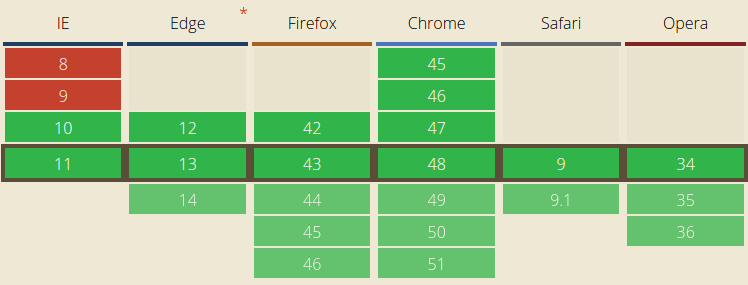
\includegraphics[height=5cm,width=11cm]{img/appCache-support.png}
		\\
		
\includegraphics[height=0.5cm,width=5cm]{img/legende.png}
	\end{center}
\end{frame}